\subsection{Climate and Production}

\subsubsection{Climate Change Trend}
\begin{figure}[ht]
    \centering
    \caption{Average Temperature since 1990 to 2021} 
    \label{fig:trend_avg_temp}
    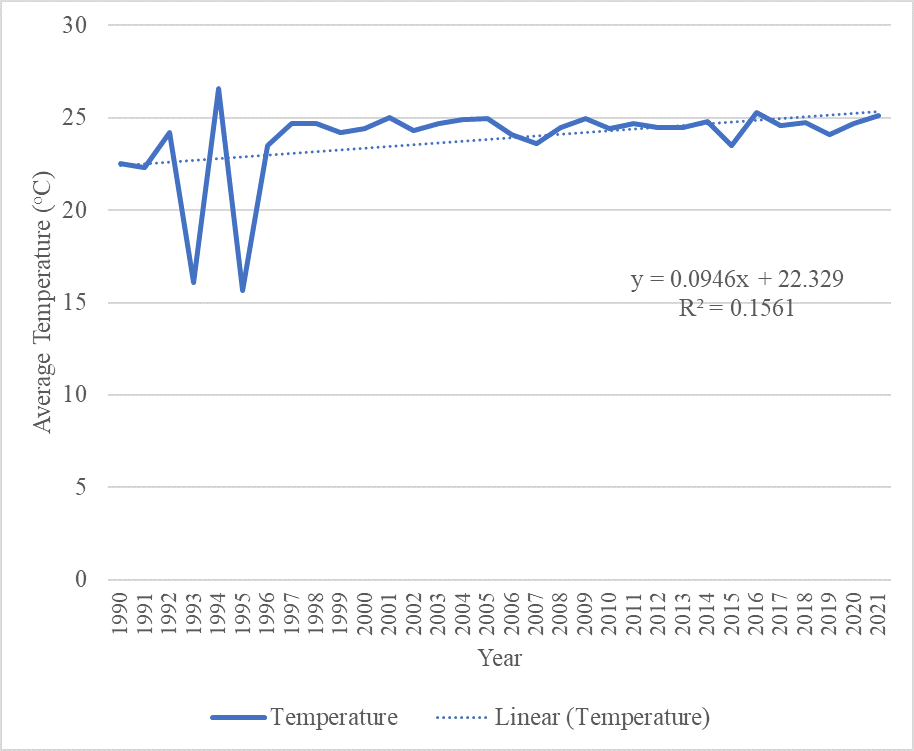
\includegraphics[width=0.9\textwidth]{images/trend_avg_temp.png}
\end{figure}

As shown in Figure~\ref{fig:trend_avg_temp}, the results indicate


\subsection{Correlation Between Yield and Climate Variables}


% Correlation Table
\begin{table}[h]
    \centering
    \caption{Correlation Table between Yield and Climate Variables}
    \resizebox{\textwidth}{!}{ % Resize table to fit within text width
    \begin{tabular}{lccc}
        \toprule
        & \textbf{Sunshine Hours} & \textbf{Accumulated Rainfall (mm)} & \textbf{Average Temperature (°C)} \\
        \midrule
        \textbf{Yield (mt/ha)} & 0.417* & -0.074 & 0.287 \\
        \textbf{(p-value)} & 0.017 & 0.686 & 0.112 \\
        \bottomrule
    \end{tabular}
    }
\end{table}

% Linear Regression Model Summary
\begin{table}[h]
    \centering
    \caption{Linear Regression Model Summary for Yield and Climate Data}
    \begin{tabular}{lc}
        \toprule
        \textbf{Dep. Variable} & Yield \\
        \textbf{Adjusted R-squared} & 0.161 \\
        \textbf{Significance (p-value)} & 0.048 \\
        \textbf{F-statistic} & 2.981 \\
        \textbf{R-squared} & 0.242 \\
        \bottomrule
    \end{tabular}
\end{table}

% Regression Coefficient Table
\begin{table}[h]
    \centering
    \caption{Regression Coefficients for Yield and Climate Data}
    \label{reg_coef_climate_yield}
    \resizebox{\textwidth}{!}{ % Resize table to fit within text width
    \begin{tabular}{lccccc}
        \toprule
        \multirow{2}{*}{\textbf{Model}} & \multicolumn{2}{c}{\textbf{Unstandardized Coefficients}} & \textbf{Standardized} & \multirow{2}{*}{\textbf{t}} & \multirow{2}{*}{\textbf{Sig}} \\
        \cmidrule{2-3}
        & \textbf{B} & \textbf{Std. Error} & \textbf{Beta} & & \\
        \midrule
        \textbf{(Constant)} & -99.061 & 903.331 & - & -0.110 & 0.913 \\
        \textbf{Sunshine} & 0.670 & 0.291 & 0.391 & 2.306 & 0.029 \\
        \textbf{Accumulated Rainfall} & -0.279 & 0.279 & -0.168 & -0.999 & 0.326 \\
        \textbf{Average Temperature} & 43.825 & 32.148 & 0.232 & 1.363 & 0.184 \\
        \bottomrule
    \end{tabular}
    }
\end{table}

\begin{equation}
    \begin{split}
        \text{Crop Yield} &= -99.061 + 0.670 \times \text{Sunshine} \\
        &\quad - 0.279 \times \text{Accumulated Rainfall} \\
        &\quad + 43.825 \times \text{Average Temperature}
    \end{split}
\end{equation}



Table 4.1 presents the correlation between crop yield and key climate variables, including sunshine hours, accumulated rainfall, and average temperature. The results indicate:

Sunshine hours show a significant positive correlation with yield (r = 0.417, p = 0.017), suggesting that increased solar exposure contributes to higher crop productivity.
Accumulated rainfall exhibits a weak negative correlation with yield (r = -0.074, p = 0.686), indicating that rainfall variability does not have a statistically significant effect on crop production.
Average temperature has a moderate positive correlation with yield (r = 0.287, p = 0.112), although the relationship is not statistically significant.
These findings suggest that sunshine hours play a more influential role in determining crop yield than rainfall or temperature variations.

Linear Regression Analysis
The linear regression model for yield and climate variables reveals an R-squared value of 0.242, indicating that approximately 24.2\% of the variability in crop yield can be explained by sunshine hours, accumulated rainfall, and average temperature. The adjusted R-squared value of 0.161 suggests a moderate explanatory power after adjusting for the number of predictors.

The regression model equation derived from the analysis is:


Regression Coefficients and Statistical Significance
Examining the individual regression coefficients:

Sunshine hours \(\beta = 0.391, \, p = 0.029\) show a significant positive effect on yield, confirming that increased sunlight exposure enhances productivity.
Accumulated rainfall \(\beta = -0.168, \, p = 0.326\) has a negative but non-significant effect, indicating that excessive or inconsistent rainfall does not significantly contribute to yield improvement.
Average temperature \(\beta = 0.232, \, p = 0.184\) has a positive but non-significant effect, suggesting that temperature variations alone are not a strong predictor of yield changes.
Discussion
Influence of Climate Factors on Crop Yield
The findings in Table \ref{reg_coef_climate_yield} indicate that sunshine hours are the most influential climate variable affecting crop yield. The significant positive correlation and regression coefficient confirm that higher solar radiation enhances photosynthesis, leading to better crop growth and productivity. This aligns with prior studies conducted in Nepal and South Asia, which found that solar radiation is a key determinant of agricultural output (Thapa \& Devkota, 2016).

Conversely, rainfall does not show a significant impact on yield, which may be due to erratic precipitation patterns in the Banke district. Similar studies in Nepal have reported that uneven rainfall distribution can reduce soil moisture availability, affecting crop health despite high total precipitation levels (Regmi et al., 2019). This suggests that rainfall variability, rather than total rainfall, may be more critical for crop yield determination.

The moderate but non-significant relationship between temperature and yield suggests that while temperature fluctuations impact crop growth, their effect is less direct than sunshine exposure. Previous research has found that higher temperatures may accelerate crop maturation but also increase evapotranspiration, reducing soil moisture levels and affecting plant growth (Shrestha et al., 2022). This could explain why the temperature variable, though positively correlated with yield, does not exhibit strong statistical significance.

Comparing with Previous Studies
Compared to previous studies in Nepal’s Terai region:

Devkota \& Paija (2020) found that a 1% increase in rainfall improved rice yield by 0.45%, while this study indicates a negative but weak relationship between rainfall and yield. The inconsistency may stem from differences in soil properties, irrigation availability, and crop types across districts.
Karki et al. (2021) reported that sunshine hours significantly influenced wheat productivity, supporting this study’s findings that higher solar exposure enhances crop output.
Risal et al. (2022) noted that temperature increases beyond optimal thresholds negatively impact yield, whereas this study does not find a strong negative effect, possibly due to regional climate adaptations.
Implications for Agricultural Adaptation Strategies
The results underscore the importance of optimizing sunshine exposure through improved crop management techniques such as:
Selecting drought-resistant crop varieties that can capitalize on high sunlight conditions.
Enhancing irrigation infrastructure to mitigate the negative impacts of inconsistent rainfall.
Adopting precision agriculture technologies to optimize planting schedules based on temperature and solar radiation patterns.

Additionally, policymakers should focus on climate-resilient agricultural practices, particularly in districts like Banke, where rainfall unpredictability poses challenges for farmers.

Limitations \& Future Research Directions
Although this study provides valuable insights, some limitations should be considered:

The relatively low R-squared value (0.242) suggests that other non-climatic factors (e.g., soil quality, pest outbreaks, irrigation methods) also influence yield and should be included in future models.
The study does not account for extreme weather events (e.g., floods, droughts), which could significantly affect yield trends.
Future research should incorporate long-term climate projections and soil moisture analysis to improve yield prediction accuracy.
Conclusion
This study highlights the strong positive impact of sunshine hours on crop yield, while rainfall and temperature have weaker, non-significant effects. The findings suggest that improving water management and leveraging sunshine exposure are key to sustaining agricultural productivity in Nepal’s Banke district. Future studies should integrate broader climate and agronomic factors to develop more comprehensive yield forecasting models.




 